% !TEX spellcheck = en_US
% !TeX root = Lecture.tex
%---------------------------------------------------------------------------------
\section[Conclusion]{Conclusion and Learning Objectives}\label{sec:CNO}
%---------------------------------------------------------------------------------
\miniframesoff	
\begin{frame}<handout:0>[noframenumbering]{Content}
\tableofcontents[currentsection]
\PutAt<1-|handout:0>[5cm]{(10cm,2cm)}{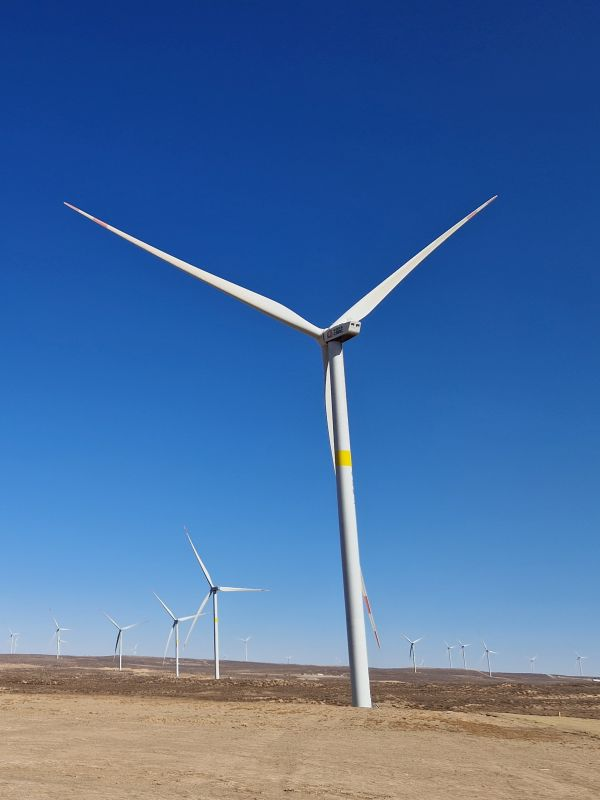
\includegraphics[width=4.0cm]{\StylePath/content/Gobi}} % graphic related to topic	
\end{frame}
\miniframeson
%---------------------------------------------------------------------------------
\begin{frame}{Conclusion}  	
	\begin{alertblock}{Main questions today}
		\begin{itemize}
			\item How much wind energy can be extracted theoretically by a wind turbine?
			\item How does this help us to design an optimal wind turbine blade?	
		\end{itemize}
	\end{alertblock}		
	\begin{block}<1->{According to Betz, the maximum power coefficient is 16/27, around 59 \%}
  		\begin{itemize}
  			\item power coefficient is ratio of extracted power to wind power 
    		\item wind power proportional to cubic wind speed, air density, rotor area 
    		\item Betz's law derived by energy balance in stream tube with divergent streamlines and Froude-Rankine Theorem    		
		\end{itemize}
	\end{block}	
	  	\begin{block}<2->{Blade design according to Betz}
	  		\begin{itemize}
	    		\item inputs: number of blades, rotor radius, tip speed ratio, angle of attack, lift coefficient
	    		\item output: distribution of chord length and twist angle
	  			\item no losses are considered, so it is not very realistic, but a good starting point	    		
			\end{itemize}
		\end{block}			
\end{frame}
%---------------------------------------------------------------------------------
\begin{frame}{Learning objectives}  	
\begin{block}{After this lectures you should be able to...}
	\begin{itemize}
		\item explain, how much kinetic energy is in the wind and which maximum fraction of this energy can be converted to mechanical energy
		\item derive the maximum power coefficient according to Betz
		\item select values for rotor design from an airfoil
		\item design a rotor according to Betz
	\end{itemize}
\end{block}
\end{frame}
%---------------------------------------------------------------------------------
%---------------------------------------------------------------------------------
\begin{frame}{References}
%\renewcommand{\bibfont}{\tiny}%\fontsize{6}{6}\selectfont
\printbibliography[heading=none]
\end{frame}
%---------------------------------------------------------------------------------
